\documentclass[12pt]{article}
\usepackage[english]{babel}
\usepackage[table,xcdraw]{xcolor}
\usepackage{booktabs}
\usepackage{tabularx}
\usepackage{enumerate}
\usepackage{graphicx}
\usepackage[section]{placeins}
\usepackage{float}
\usepackage{url}
\usepackage{wrapfig}
\usepackage[toc,page]{appendix}
\usepackage{caption}
\usepackage{enumitem}
\usepackage[style=numeric-comp, sorting=none]{biblatex}
\usepackage{pdflscape}
\usepackage{adjustbox}
\usepackage{csquotes}
\usepackage{hhline} % for double lines
\usepackage{listings}
\usepackage{hyperref}
\pagestyle{plain}


\captionsetup{justification=centering}

\graphicspath{{images/}}
\bibliography{refs.bib}

\begin{document}

\begin{titlepage}

\newcommand{\HRule}{\rule{\linewidth}{0.5mm}} % Defines a new command for the horizontal lines, change thickness here

\center % Center everything on the page
 
%----------------------------------------------------------------------------------------
%	HEADING SECTIONS
%----------------------------------------------------------------------------------------

\textsc{\LARGE Universitat Politècnica de Catalunya}\\[1.5cm] % Name of your university/college
\textsc{\Large Algorithms, Data Structures and Databases}\\[0.5cm] % Major heading such as course name

%----------------------------------------------------------------------------------------
%	TITLE SECTION
%----------------------------------------------------------------------------------------

\HRule \\[0.4cm]
{ \huge \bfseries Deliverable 1}\\[0.4cm] % Title of your document
\HRule \\[1.0cm]
 
%----------------------------------------------------------------------------------------
%	AUTHOR SECTION
%----------------------------------------------------------------------------------------

\begin{minipage}{0.53\textwidth}
\large
\centering
\emph{Autors}\\
Aguilera Pilo \textsc{Carles}\\
Delgado Jimenez \textsc{Joel}\\
Vilella Jam \textsc{Oriol}\\
\end{minipage}
~
\begin{minipage}{0.4\textwidth}
\end{minipage}\\[2cm]

% If you don't want a supervisor, uncomment the two lines below and remove the section above
%\Large \emph{Author:}\\
%John \textsc{Smith}\\[3cm] % Your name

%----------------------------------------------------------------------------------------
%	DATE SECTION
%----------------------------------------------------------------------------------------

{\large \today}\\[2cm] % Date, change the \today to a set date if you want to be precise

%----------------------------------------------------------------------------------------
%	LOGO SECTION
%----------------------------------------------------------------------------------------


\includegraphics[scale=0.3]{logo-upc.png}\\[1cm]
 
%----------------------------------------------------------------------------------------

\vfill % Fill the rest of the page with whitespace

\end{titlepage}

\newpage

\tableofcontents
\thispagestyle{empty}


\newpage

\pagenumbering{arabic}

\newpage

\section{Instructions}

\subsection{Environment}
The project requires the following environment variables to be defined:
\begin{itemize}
    \item ACCESS\_KEY\_ID
    \item SECRET\_ACCESS\_KEY
    \item S3\_API\_ENDPOINT
    \item S3\_CONSOLE\_ENDPOINT
    \item CHROMADB\_ENDPOINT
    \item CHROMADB\_PORT
    \item GEMINI\_API\_KEY
\end{itemize}
These should be provided in and env file. An example can be found in the repository in a file named \textit{env.example}.

Gemini API Key can be obtained easily and free through Google AI Studio\footnote{https://aistudio.google.com/}.

\subsection{Deployment}
The project consists of two distinguished components: The pipeline and the app.

The pipeline can be deployed using docker compose. To achieve it, execute the following command from the project's root directory:

Once the pipeline has been deployed, the app can be deployed and will work correctly. To achieve it, execute the following command (also from the project's root directory):



\newpage

\section{Context \& Data}

\subsection{Context}
The domain chosen for this is within the healthcare sector, specifically focusing on the detection and analysis of \textbf{skin cancer}.

We believe the current exponential growth of technology offers significant potential for application across multiple sectors, particularly in health and human well-being. This justifies our choice of domain: the development of technological tools aimed at the prediction and detection of skin cancer.

In recent years, the incidence of this disease has increased significantly, primarily due to greater public sun exposure. We therefore consider it essential to pursue data-driven and AI-based solutions that contribute to the prevention and early diagnosis of skin cancer.

As an academic project, we acknowledge this is an initial approximation. There is clear scope for future improvements, particularly concerning the model's accuracy and the quality of the data employed.

\subsection{Data}

The data for this project were primarily sourced from \textbf{Kaggle}, one of the biggest platforms in the Data Science community. This was complemented with information obtained from other open sources, such as informational websites, notably \textbf{Wikipedia}.

This are the datasets used for our project:
\begin{enumerate}
    \item \href{https://huggingface.co/datasets/abaryan/ham10000_bbox}{HAM10000 Dataset}: This dataset forms the visual part of our project. The HAM10000 dataset is a very famous and widelly used public collection of dermatoscopic images of common skin lesions, including various types of skin cancer. We load the dataset and since we can't handle all the images from the dataset, because the pipeline will be very slow, we obtain a sample of 100 images which is more than enough. This images serve as the image types of data and will be used to generate embeddings to perform similarity searches across modalities.

    \item Textual Data: This dataset proviedes the descriptive knowledge base for our project. We have implemented a \textbf{Web Scrapper} in order to scrape articles directly from Wikipedia, given some target key topics. The topics we have defined are Skin Cancer, Melanoma, Basal Cell Carcinoma, Squamous Cell Carcinoma and Actinic Keratosis. This topics can be changed at any time but the only condition is that they have to appear as a Wikipedia page. Otherwise, the scrapping will fail and it will not produce any text. 
    
    The web scrapper downloads the contents of these pages, cleans the raw HTML, and removes unnecessary elements like citation brackets. This generates our dataset which is several .txt files, one for each topic. 
    
    This text represents the descriptive modality. The embeddings generated from the text will be matched across all the embeddings we generate from the other datasets. This allows a user to search for "information about basal cell carcinoma" and get back not only this text but also related images and even audio.

    \item \href{https://huggingface.co/datasets/Moaaz55/skin_cancer_questions_answers}{Audio Data}: This is our third and last modality for this project, representing information as spoken language. In this dataset is a two-step process. We first get the content from a Hugging Face dataset containing questions and answers about skin cancer. Then, instead of using this data as text, we sample 100 of the answers from the dataset, we use a \textbf{text-to-speech} (TTS) engine to synthesize these text answers into audio. And finally we save this as individual .wav files. This creates a dataset of spoken explanations. This will allow our system to work with audio as a distinct modality. We -will generate embeddings out of this audio in order to perform similarity searches across modalities.
\end{enumerate}

All this data is collected automatically by a script. This script, although we consider it does not belong to the pipeline (since the pipeline officially starts once the data is uploaded ot the temporal landing zone), is executed at the beginning just before the Temporal Landing Zone. That is because we wanted to automate it. However, in a real case scenario we would configure datasources to send data directly to MinIO. 

\section{Data Management Backbone}

This section describes the project's data zones and the design decisions implemented for data handling and processing.

We have employed \textbf{MinIO} as our object storage system, creating a separate bucket for each layer or zone of the project. All objects are first loaded into the Temporal Landing Zone in their raw, original format, with no structure or pre-processing. The objective of this layer is to ensure rapid and complete data ingestion.

In the other layers, the buckets are organized and structured by data modality (images, text and audio). This approach allows us to maintain a clear, consistent, and more manageable data structure.

This layered architecture enables us to effectively track the data pipeline's evolution and visualitze the transformations applied to the data thoughout the entire process.

\subsection{Software Architecture}

\subsection{Landing Zone}

This project layer, the \textbf{Landing Zone}, is divided into two distinct sub-zones: the Temporal Landing Zone and the Persistent Landing Zone.

The first, the \textbf{Temporal Landing Zone}, serves as the initial data ingestion or staging area. It acts as a data lake where all objects are uploaded in their raw original format, without any transformation.

The second, the \textbf{Persistent Landing Zone}, is where we begin to structure and organize the data. In this phase, we classify objects based on their modality (images, text or audio) and store them in their corresponding locations.

This initial organization ensures the data is correctly partitioned and prepared for subsequent processing stages.

\subsubsection{Temporal Zone}

As explained in the introductory section, this phase involves loading data from our various origin sources directly into MinIO. This ingestion allows us to capture all data within the bucket in its original, unaltered format.

\begin{figure}[H]
    \centering
    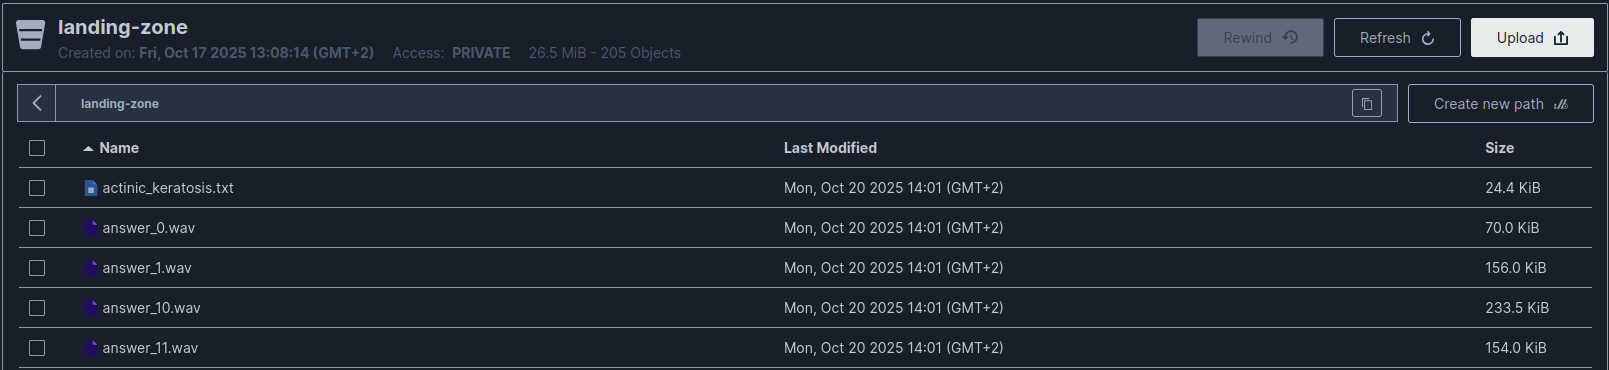
\includegraphics[width=1\linewidth]{temporal.png}
    \caption{Temporal Landing Zone}
    \label{fig:temporal}
\end{figure}

\subsubsection{Persistent Zone}

In this layer, we organized the objects and elements to simplify subsequent management and processing. To achieve this, we created a separate folder for each data type: one for images, one for text, and another for audio. This classification allows us to treat each data type differently and maintain a coherent structure with our data.


\begin{figure}[H]
    \centering
    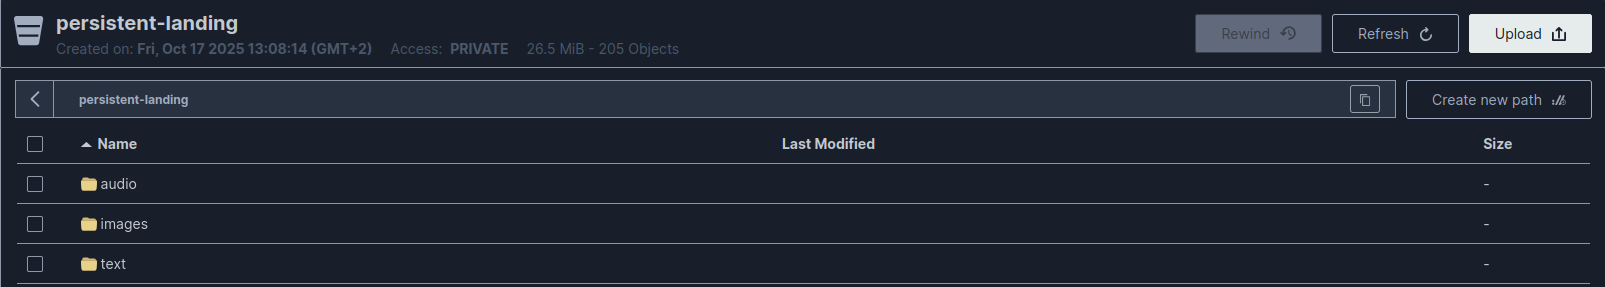
\includegraphics[width=1\linewidth]{persistent.png}
    \caption{Persistent Landing Zone}
    \label{fig:persistent}
\end{figure}

\subsection{Formatted Zone}
Until now tha data only has been classified according to its modality. In this layer, the data is preprocessed to ensure all elements are in a homogeneous format and a coherent structure. However, notice that the content is not altered: All the transformations are only format-wise.

Initially, we evaluated assigning a unique identifier (ID) to each object in order to facilitate traceability and searches. However, this option was discarded as the point of this project is to leverage the advantages of embeddings to retrieve similar elements.

In the end, for the scope of this project we have considered it is not needed to provide any metadata beyond the original filenames as the primary identifiers. So, in this zone we ensure format consistency between all of them, depending on their modality:
\begin{itemize}
    \item \textbf{Texts}: Normalized to \textbf{.txt}
    \item \textbf{Images}: Normalized to \textbf{.png}
    \item \textbf{Audios}: Normalized to \textbf{.mp3}
\end{itemize}

These formats were chosen as the most suitable standards for each modality, due to being very well-known formats. However, these could be changed if it was needed.

\begin{figure}[H]
    \centering
    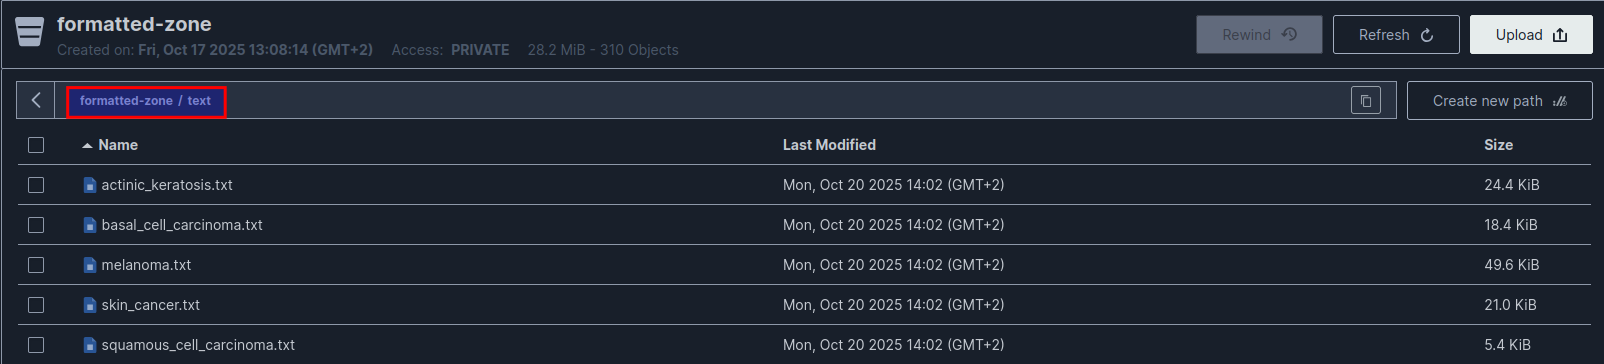
\includegraphics[width=1\linewidth]{images/formatted-text.png}
    \caption{Text format unified}
    \label{fig:placeholder}
\end{figure}

\begin{figure}[H]
    \centering
    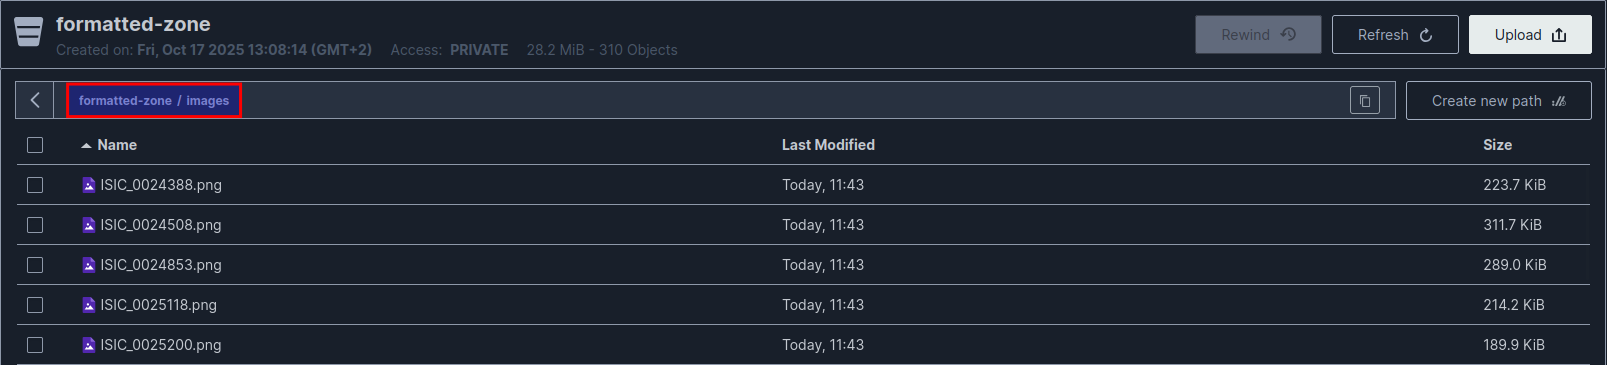
\includegraphics[width=1\linewidth]{images/formatted-images.png}
    \caption{Image format unified}
    \label{fig:image}
\end{figure}

\begin{figure}[H]
    \centering
    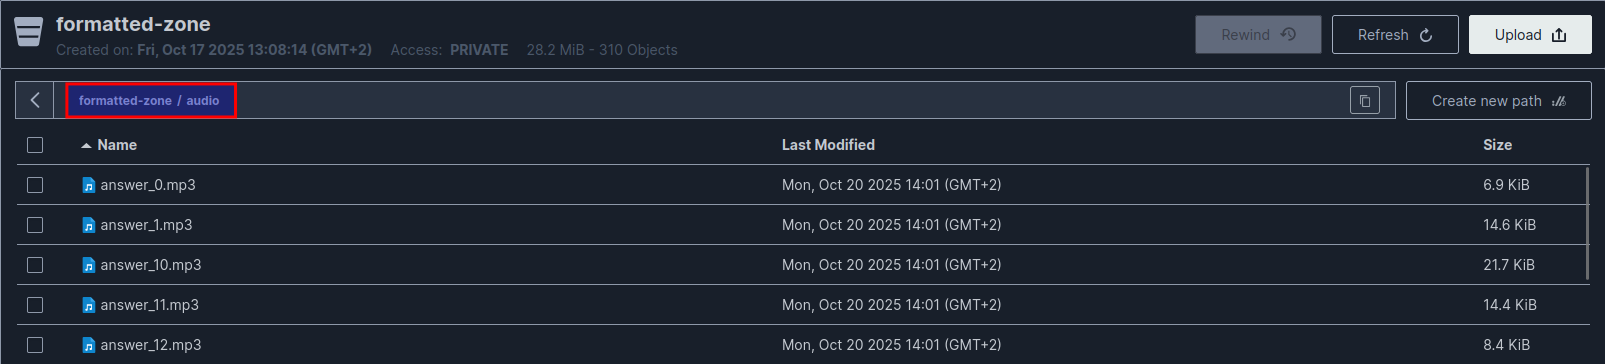
\includegraphics[width=1\linewidth]{images/formatted-audio.png}
    \caption{Audio format unified}
    \label{fig:placeholder}
\end{figure}

\subsection{Trusted Zone}
In this phase, we process all content (images, audio and text) to ensure it is clean, standardized, and ready for use in the last stage of the pipeline. Therefore, the trusted zone contains all the data after applying a sequence of generic transformations trying to prepare the data without adhering to the specific requirements of an specific model (that will be explained in the exploitation zone). 

At the beginning, we realized an analysis to identify the format and status of the data within each of three modalities. This provided a general overview of the quality of the objects and characteristics, allowing us to proceed with a specific processing method for each data type. In addition, a data analysis and preprocessing stage was carried out to examine their characteristics.
The quality report for each element can be viewed in the repository, inside the notebooks folder located within the trusted-zone directory, or directly through the front-end in the “Quality Report” tab.

Since the number of actions performed for each modality is larger than in previous cases, they are detailed in the subsections below:

\subsubsection{Image Processing}
Images are extracted from the Formatted Zone, processed, and then stored in the Trusted Zone. The process applies different measures to enhance visual quality:
\begin{itemize}
    \item Resize to uniform 600x450 pixels shape to ensure consistency.
    \item RGB Conversion for compatibility with further stages of the pipeline.
    \item 10\% increase in brigthness for clearer images.
    \item 15\% increase in contrast to highlight details.
    \item 5\% increase in saturation to make colors more vibrant.
    \item Light Gaussian blur to reduce digital noise. This softening was then compensated for withsharpening filter to restore detail and maintain image clarity.
\end{itemize}

These are a set of transformations that we have considered suitable for improving the visual quality of these images for better use in the future. The values such as the percentages have been arbitrarily decided as an example.

\subsubsection{Text Processing}
The text preprocessing stage aims to clean, normalize, and standardize all text files before their integration into the analysis pipeline.
This phase ensures that textual content is coherent, readable, and noise-free, facilitating its subsequent indexing and embedding generation.

The main operations performed are as follows:

\begin{itemize}
    \item Unicode normalization (NFKD) to unify special characters, accents, and non-standard symbols.
\end{itemize}

\begin{itemize}
    \item Removal of control and non-printable characters, preserving only relevant line breaks and tabulations.
\end{itemize}

\begin{itemize}
    \item Reduction of multiple white spaces, converting sequences of spaces or tabs into a single space.
\end{itemize}

\begin{itemize}
    \item Simplification of line breaks, limiting empty lines to a maximum of two consecutive ones.
\end{itemize}

\begin{itemize}
    \item Trimming of leading and trailing spaces on each line to maintain a clean and uniform structure.
\end{itemize}

\begin{itemize}
    \item Removal of unnecessary empty lines, both at the beginning and end of the text.
\end{itemize}

\begin{itemize}
    \item Cleaning of problematic special characters, keeping only standard punctuation and alphanumeric symbols.
\end{itemize}

\begin{itemize}
    \item Normalization of quotation marks and apostrophes, converting typographic versions into straight quotes (" and ').
\end{itemize}

\begin{itemize}
    \item Unification of multiple hyphens, reducing sequences of -- or more into a single hyphen (-).
\end{itemize}

\begin{itemize}
    \item Normalization of spacing around punctuation, removing unnecessary spaces before punctuation marks and ensuring a single space after them.
\end{itemize}

\begin{itemize}
    \item Final trimming of leading and trailing spaces in the entire text.
\end{itemize}

\begin{itemize}
    \item Content verification to ensure that the resulting file is not empty after processing.
\end{itemize}

Finally, the cleaned text is saved in UTF-8 format and uploaded to the trusted-zone bucket in MinIO, preserving the original structure under the text/ prefix.

This process guarantees that all text files present a consistent structure, free from residual characters and inconsistencies, and are ready for semantic processing and multimodal similarity search.

\subsubsection{Audio Processing}
The audio preprocessing stage aims to ensure the technical consistency and quality of all audio files before their integration into the analysis pipeline.
This phase applies a series of transformations to clean, normalize, and standardize the audio data, ensuring compatibility with multimodal processing models.

The main operations performed are as follows:

\begin{itemize}
    \item Sampling rate normalization to 48 kHz to unify all audio files.
\end{itemize}

\begin{itemize}
    \item Automatic silence removal at the beginning and end, detecting silent segments longer than 500 ms below –50 dB.
\end{itemize}

\begin{itemize}
    \item Volume normalization and dynamic range compression (threshold –20 dB, ratio 4:1, attack 5 ms, release 50 ms) to balance loudness levels.
\end{itemize}

\begin{itemize}
    \item Noise filtering using a high-pass filter at 80 Hz and a low-pass filter at 16 kHz to remove undesired low- and high-frequency components.
\end{itemize}

\begin{itemize}
    \item Final gain adjustment with a +2 dB amplification to enhance presence and clarity.
\end{itemize}


    Final export in MP3 format (192 kbps) and upload to the trusted-zone bucket in MinIO for further indexing and analysis.


This process ensures that all audio files share a homogeneous format, clean sound, and optimal quality for embedding extraction and multimodal similarity search.

\section{Exploitation Zone}
The exploitation zone is that zone from our pipeline where we actually process our data according to the requirements of an specific task. In our case, the primary objective of this zone is to take the different supported modalities of data (images, text and audio) and extract their embeddings in a \textbf{unified} space. The aim of this process is to allow us to perform multimodal similarity searches given the user input.

\subsection{Embeddings extraction}
To achieve it, it is mandatory for the embeddings of the different modalities to belong to the same embedding space. That means that all embeddings need to be generated by the same model.

We started to investigate the use of multiple compatible models such as CLIP (for image and text) and Wav2CLIP (for audio to clip), which are different models whose embeddings spaces are compatible. However, after finding Meta's \href{https://github.com/facebookresearch/ImageBind}{ImageBind} model, we ended leaning on it since it alone can embed all three data types into the same space. Also, if we used different models, we would had to embed text in more than one space (one for the similarity search across texts and another for the similarity searches across other modalities). We thought this could impact the performance of our pipeline, so we decided to keep going on using a single model to achieve everything.

In the official ImageBind documentation, the standard functions for generating embeddings require a path to a file. This limitation was not suitable for our application since that would mean that we should download each object from MinIO, store it into a temporal folder, process it and then delete it. To solve it, we observed and understood the internals of the functions provided by the model class in the public repository and, based on that, we implemented our own solution to bypass this file-path limitation.

This custom implementations allowed us to generate embeddings directly from in-memory data, which is far more suitable for our pipeline. 

\subsection{Vector database}
After generating embeddings, we insert them into our vector database for future modality searches. We use a \textbf{ChromaDB} instance deployed as a separated docker container in the same way as MinIO. 

The embeddings are stored into 3 separated collections, one for each modality. The reason why we have decided this is to logically separate it and facilitate the implementation of "similar modality seaches" (task 1). For multimodal searches we will have to query all the collections to retrieve all data from all supported types.

\subsection{Particular case: Text transformation}
After doing the first proof of concept, we notices ImageBind model has an input limit for texts of 100 tokens approximately. If the input length is greater, the generated embeddings will be the same and the user input will be at the same distance from all the other texts. To avoid this situation, it is needed to partition our texts into smaller fragments.

After thinking about in which phase should we apply this transformation, we finally decided to apply it in the transition from the trusted zone to the exploitation zone. That is because this transformation is imposed by the specific requirements of our model. In other words, it is a very ad-hoc treatment (other models may not require it). We believe trusted zone should contain clean data in a generic way that is independent from the specific needs of models (analytical backbone). Therefore, we have ended applying it there, just before generating the embeddings.

\section{Application development: Chatbot}
The final part of our project is the development of a user interface chatbot-like that allows a user to perform any of the following 3 tasks:
\begin{itemize}
    \item Task 1. Similar modality search
    \item Task 2. Multimodal similarity search
    \item Task 3. RAG with external LLM
\end{itemize}

The user interface is based on Streamlit\footnote{https://streamlit.io/}, an open-source Python framework for delivering interactive Machine Learning and Data Science applications. 

\subsection{Task 1. Similar modality search}
This modality corresponds to Task 1, and its purpose is to, given a specific input object, return the most similar elements to the one provided.
For example, if an image of skin cancer or melanoma is given, the system will return the images that are most similar to the one provided as input.

The same process applies to other types of data, such as texts or audio. By providing a specific input through the prompt in the front-end, the task retrieves and returns the most similar elements of the same type (image, text, or audio).

The process works as follows:
when an object arrives from the front-end, it is processed through the pipeline without being uploaded to MinIO first. The goal is to obtain an object with the same format as those already stored in MinIO, from which embeddings have been generated.
This new element is transformed so that, when its embedding is created, it is as representative and realistic as possible. This allows us to compare it with the embeddings already stored in ChromaDB and identify which items in the database are the most similar.

This procedure is applied to all types of elements, and the front-end allows users to select the desired modality, audio, text, or image.

Finally, a K value is included to specify the number of output results to be returned, for example, 1, 2, 10, or any number required.
\subsection{Task 2. Multimodal similarity search}
In this second task, we implemented the multimodal similarity search.

The main objective of this task is to enable the system, given a specific query, to provide a richer and more comprehensive response by combining different types of data.
Although it does not reach the level of reasoning and generation achieved in Task 3, this stage already allows, from a single input, the retrieval of information across multiple modalities (text, image, and audio).

For example, when providing the text “What is skin cancer”, the system returns both the most similar texts related to skin cancer and the most relevant images associated with it. This behavior can be extended to any combination of input and output modalities, text, image, or audio.

The most significant challenge of this task was ensuring that all object types (images, texts, and audio) had embeddings projected into a shared multidimensional space.
This allows an input text to be compared not only with textual embeddings but also with image and audio embeddings, by computing the minimum distance within this common space and retrieving the most similar elements based on semantic proximity.

Initially, handling images and texts posed no major issues, as we used the CLIP library together with ChromaDB to generate embeddings and perform similarity comparisons.
However, the main difficulty arose when integrating audio data, since CLIP does not natively support audio embeddings. To address this, we explored several alternatives that could generate audio embeddings within the same latent space as CLIP’s text and image embeddings.

Among the solutions tested were Wav2CLIP and LAION-CLAP, but the results were unsatisfactory: many implementations were deprecated, unstable, or incompatible with CLIP’s multidimensional space.
Due to these limitations, we ultimately decided to migrate to Meta’s ImageBind library, which allows generating text, image, and audio embeddings within a unified multimodal space.
We installed Meta’s official ImageBind repository and integrated it into our processing pipeline, successfully achieving a shared embedding space for all object types, enabling an effective multimodal similarity search system.

\subsection{Task 3. RAG with external LLM}
This task can be viewed as performing task 2 and then sending a query to an external LLM. At first, we tried to do a proof of concept by deploying LLaVA model locally, but we discarded it as we had some difficulties related with the size of the model. We opted for using Gemini API through the Python official SDK, as it is a well-known LLM and its free tier is enough for our needs and allows us to send multimodal queries involving images, texts and audios. Some of the avantages of using Gemini are the easy integration for quick tests and not having to have the infraestructure to deploy the model. Nevertheless, some of the drawbacks are the economic cost (it it were deployed in a real case scenario, the free tier would very likely not be enough), loose of privacy and the loss of control on the model training (since it is deployed on Google's infraestructure).

Currently, due to some difficulties managing multiple inputs, task 3 only accepts text and one image as user input. After that, the application queries ChromaDB for the related texts and images, crafts and enhanced prompt, sends it to Gemini and shows the response through the user interface. Notice that the number of retrieved results is equal to the dot product of the number of elements and number of types of data. In other words:
\begin{itemize}
    \item If the user sends a text, the system will query for the most similar text and the most similar image.
    \item If the user send a text and image, the system will query for the most similar text and the most similar image for the given text, and also will query for the most similar text and the most similar image for the given image. So , in total, 2 texts and 2 images would be sent as context to the LLM.
\end{itemize}

The current approximation presents some drawbacks: From one hand, we are not benefitting from audio information, since we are ignoring it. We have done that in order to control the number of files that we send to the external LLM. From the other hand, we are limiting the user to only be able to upload one image for prompt  


\end{document}
